\section{Dynamische Schriften}
\label{sec:editor-obj-dynstr}

\begin{figure}[h]
\centering
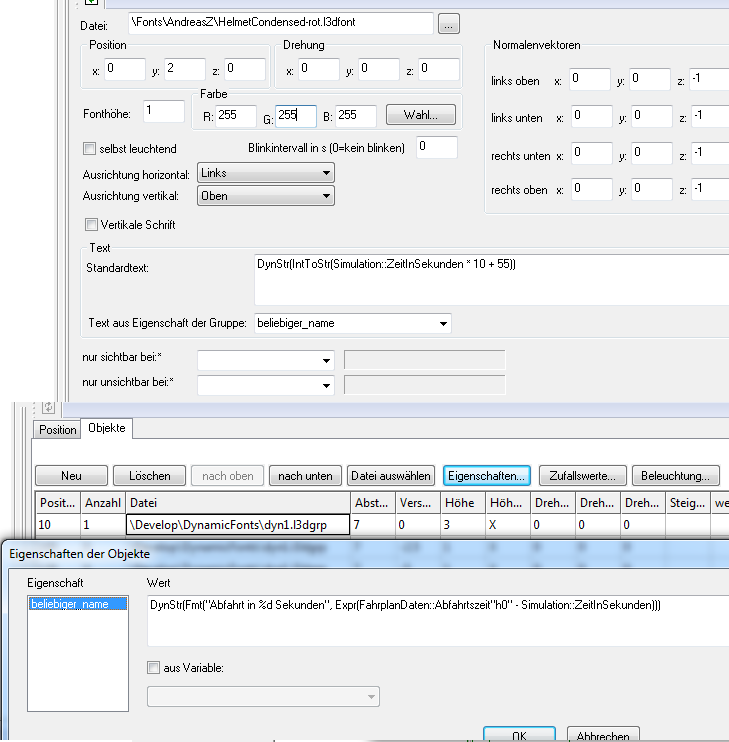
\includegraphics[width=1.0\textwidth]{editor/images/dynamische_schrift.png}
\caption{Möglichkeiten dynamische Schriften zu setzen (oben Gruppenobjekt, unten Streckeneditor)}
\label{fig:editor:dynstr}
\end{figure}

Mit dynamischen Schrifte ist es möglich, den Inhalt von Fonts dynamisch
oder anhand statischer Variablen zu steuern.

Die Ausdrücke können dabei als Standardtext bei Fonts in Gruppenobjekten
eingestellt werden. Oder man setzt den entsprechenden Ausdruck im
Streckeneditor über die Eigenschaften des Objekts.

Dynamische Schriften haben immer die Form \texttt{DynStr()}. Abbildung \ref{fig:editor:dynstr} zeigt zwei Beispiele für die Möglichkeiten Dynamischen Schriften zu definieren.

\subsection{Syntax in EBNF}

Eine Beschreibung der EBNF ist in der \href{http://de.wikipedia.org/wiki/EBNF}{Wikipedia} verfügbar.

\begin{longtable}[c]{@{}lll@{}}
\hline\noalign{\medskip}
\begin{minipage}[t]{0.22\columnwidth}\raggedright
dyn\_font\_expr
\end{minipage} & \begin{minipage}[t]{0.06\columnwidth}\raggedright
=
\end{minipage} & \begin{minipage}[t]{0.73\columnwidth}\raggedright
'DynStr(', func, ')';
\end{minipage}
\\\noalign{\medskip}
\begin{minipage}[t]{0.17\columnwidth}\raggedright
func
\end{minipage} & \begin{minipage}[t]{0.06\columnwidth}\raggedright
=
\end{minipage} & \begin{minipage}[t]{0.78\columnwidth}\raggedright
strarg \textbar{} strfmt \textbar{} expr;
\end{minipage}
\\\noalign{\medskip}
\begin{minipage}[t]{0.17\columnwidth}\raggedright
strarg
\end{minipage} & \begin{minipage}[t]{0.06\columnwidth}\raggedright
=
\end{minipage} & \begin{minipage}[t]{0.78\columnwidth}\raggedright
'FahrplanVars::', var\_chars \textbar{} 'WetterVars::', var\_chars
\textbar{} 'FahrplanDaten::NextHalt("', halt\_chars, '")' \textbar{} 'FahrplanDaten::LastHalt' \textbar{} 'Str::', var\_chars;
\end{minipage}
\\\noalign{\medskip}
\begin{minipage}[t]{0.17\columnwidth}\raggedright
strfmt
\end{minipage} & \begin{minipage}[t]{0.06\columnwidth}\raggedright
=
\end{minipage} & \begin{minipage}[t]{0.78\columnwidth}\raggedright
'Fmt('", fmt\_chars, '",' func\_args, ')';
\end{minipage}
\\\noalign{\medskip}
\begin{minipage}[t]{0.17\columnwidth}\raggedright
func\_args
\end{minipage} & \begin{minipage}[t]{0.06\columnwidth}\raggedright
=
\end{minipage} & \begin{minipage}[t]{0.78\columnwidth}\raggedright
func\_args, ',' , func \textbar{} func;
\end{minipage}
\\\noalign{\medskip}
\begin{minipage}[t]{0.17\columnwidth}\raggedright
expr
\end{minipage} & \begin{minipage}[t]{0.06\columnwidth}\raggedright
=
\end{minipage} & \begin{minipage}[t]{0.78\columnwidth}\raggedright
'Expr(', logic\_expr , ')';
\end{minipage}
\\\noalign{\medskip}
\begin{minipage}[t]{0.17\columnwidth}\raggedright
logic\_expr
\end{minipage} & \begin{minipage}[t]{0.06\columnwidth}\raggedright
=
\end{minipage} & \begin{minipage}[t]{0.78\columnwidth}\raggedright
Ausdruck dynamische Sichtbarkeitssteuerung
\end{minipage}
\\\noalign{\medskip}
\begin{minipage}[t]{0.17\columnwidth}\raggedright
var\_chars
\end{minipage} & \begin{minipage}[t]{0.06\columnwidth}\raggedright
=
\end{minipage} & \begin{minipage}[t]{0.78\columnwidth}\raggedright
Gültiger Variablennamen
\end{minipage}
\\\noalign{\medskip}
\begin{minipage}[t]{0.17\columnwidth}\raggedright
fmt\_chars
\end{minipage} & \begin{minipage}[t]{0.06\columnwidth}\raggedright
=
\end{minipage} & \begin{minipage}[t]{0.78\columnwidth}\raggedright
Gültiger printf Format-String
\end{minipage}
\\\noalign{\medskip}
\begin{minipage}[t]{0.17\columnwidth}\raggedright
halt\_chars
\end{minipage} & \begin{minipage}[t]{0.06\columnwidth}\raggedright
=
\end{minipage} & \begin{minipage}[t]{0.78\columnwidth}\raggedright
Gültiger Haltname, Etwaige Anführungszeichen '' im Haltnamen müssen durch \textbackslash{}'' ersetzt werden
\end{minipage}
\\\noalign{\medskip}
\hline
\noalign{\medskip}
\caption{Syntax der Dynamischen Schriften in EBNF}
\end{longtable}

\subsection{Erklärung}

Die einfachsten dynamischen Schriften greifen schlicht auf Wetter- oder
Fahrplanvariablen zu. Dies geschieht mit der gleichen Syntax wie in
\hyperref[sec.editor.obj.logischeausdruecke]{Logischen Ausdrücken}.

Möchte man eine Zahl darstellen, kann man dies mittels der \texttt{Expr}
Funktion erledigen. Als Argument kann dieser Funktion jeder gültige
Logische Ausdruck übergeben werden. Das numerische Ergebnis des
logischen Ausdrucks, wird in einen String im Dezimalsystem umgewandelt.

Die komplexeste Art von dynamischen Schriften beinhalten den Aufruf der
Funktion \texttt{Fmt}. Diese ermöglicht es, einen komplexen
Ergebnisstring zu erstellen. Als erstes Argument muss dieser Funktion
ein Format-String übergeben werden, welcher bestimmt wie das Ergebnis
zusammengesetzt wird. Dabei können die \href{http://en.wikipedia.org/wiki/Printf#Format_placeholders}{Formatierungsoptionen
von printf} verwendet werden. Danach werden die Argumente für die
Formatierungsplatzhalter übergeben. Es kann hier entweder ein Zugriff
auf eine Variable erfolgen, ein logischer Ausdruck in der Form
\texttt{Expr()} angegeben werden oder wiederum eine Fmt Funktion
verwendet werden.

Zur Verdeutlichung einige Bespiele für mögliche Formatanweisungen.
Leerzeichen wurden dabei durch \emph{␣} ersetzt. Es wird angenommen,
dass \emph{FahrplanVars::h} im Fahrplan als \emph{halt} definiert ist.

\label{sec:editor-obj-dynstr-params}
Ähnlich wie bei der Sichtbarkeitssteuerung können in dynamischen Schriften Variablen in der Form \emph{Str::xxx} verwendet werden. Diese können dann über die Objekteigenschaften im Streckeneditor gesetzt werden. Beim Setzen solcher Eigenschaften kann entweder eine fixe Zeichenkette oder wiederum eine dynamische Schrift in der Form \emph{DynStr(...)} verwendet werden. Wird die Variable in einem verschachtelten logischen Ausdruck verwendet, können die Eigenschaften in der gleichen Art wie bei der Sichtbarkeitssteuerung gesetzt werden.\abversion{2.9}

\begin{longtable}[c]{@{}ll@{}}
\hline\noalign{\medskip}
\begin{minipage}[b]{0.67\columnwidth}\raggedright
Ausdruck
\end{minipage} & \begin{minipage}[b]{0.33\columnwidth}\raggedright
Ergebnis
\end{minipage}
\\\noalign{\medskip}
\hline\noalign{\medskip}
\begin{minipage}[t]{0.67\columnwidth}\raggedright
DynStr(Fmt(''aa\%daa'', Expr(10)))
\end{minipage} & \begin{minipage}[t]{0.33\columnwidth}\raggedright
aa10aa
\end{minipage}
\\\noalign{\medskip}
\begin{minipage}[t]{0.67\columnwidth}\raggedright
DynStr(Fmt(''aa\%4daa'', Expr(10)))
\end{minipage} & \begin{minipage}[t]{0.33\columnwidth}\raggedright
aa␣␣10aa
\end{minipage}
\\\noalign{\medskip}
\begin{minipage}[t]{0.67\columnwidth}\raggedright
DynStr(Fmt(''aa\%4daa'', Expr(1000)))
\end{minipage} & \begin{minipage}[t]{0.33\columnwidth}\raggedright
aa1000aa
\end{minipage}
\\\noalign{\medskip}
\begin{minipage}[t]{0.67\columnwidth}\raggedright
DynStr(Fmt(''aa\%-4daa'', Expr(1)))
\end{minipage} & \begin{minipage}[t]{0.33\columnwidth}\raggedright
aa1␣␣␣aa
\end{minipage}
\\\noalign{\medskip}
\begin{minipage}[t]{0.67\columnwidth}\raggedright
DynStr(Fmt(''aa\%-4daa'', Expr(1234)))
\end{minipage} & \begin{minipage}[t]{0.33\columnwidth}\raggedright
aa1234aa
\end{minipage}
\\\noalign{\medskip}
\begin{minipage}[t]{0.67\columnwidth}\raggedright
DynStr(Fmt(''aa\%04daa'', Expr(2)))
\end{minipage} & \begin{minipage}[t]{0.33\columnwidth}\raggedright
aa0002aa
\end{minipage}
\\\noalign{\medskip}
\begin{minipage}[t]{0.67\columnwidth}\raggedright
DynStr(Fmt(''aa\%04daa'', Expr(11111)))
\end{minipage} & \begin{minipage}[t]{0.33\columnwidth}\raggedright
aa11111aa
\end{minipage}
\\\noalign{\medskip}
\begin{minipage}[t]{0.67\columnwidth}\raggedright
DynStr(Fmt(''aa\%-10saa'', FahrplanVars::h))
\end{minipage} & \begin{minipage}[t]{0.33\columnwidth}\raggedright
aahalt␣␣␣␣␣␣aa
\end{minipage}
\\\noalign{\medskip}
\begin{minipage}[t]{0.67\columnwidth}\raggedright
DynStr(Fmt(''aa\%8saa'', FahrplanVars::h))
\end{minipage} & \begin{minipage}[t]{0.33\columnwidth}\raggedright
aa␣␣␣␣haltaa
\end{minipage}
\\\noalign{\medskip}
\hline
\noalign{\medskip}
\caption{Beispiele für Formatanweisungen}
\end{longtable}

\texttt{FahrplanDaten::NextHalt("")} liefert den nächsten Halt
\emph{nach} halt. Kommt in halt ein Anführungszeichen '' vor, muss dieses durch \textbackslash{}'' ersetzt werden.

\texttt{FahrplanDaten::LastHalt} liefert den letzten Halt der keine Betriebsstelle ist

\subsection{Performance}

Schriften die sich sehr oft ändern, sollten mit Bedacht eingesetzt
werden, da sie die fps relativ stark beeinflussen.

Verwendet eine Schrift nur konstante Werte (FahrplanVars oder konstante
logische Ausdrücke) so hat diese kaum einen Einfluss auf die Performance

\subsection{Beispiele}

\begin{verbatim}
DynStr(Fmt("Abfahrt in %d Minuten",
    Expr((Funktionen::TimeDif(
    FahrplanDaten::Abfahrtszeit("h0"), 
    Simulation::ZeitInSekunden)) / 60))
\end{verbatim}

\begin{verbatim}
DynStr(Fmt("%02d:%02d:%02d", 
    Expr(Simulation::ZeitInSekunden / 60 / 60),
    Expr(Simulation::ZeitInSekunden / 60 % 60), 
    Expr(Simulation::ZeitInSekunden % 60)))
\end{verbatim}

\begin{verbatim}
DynStr(IntToStr(Simulation::ZeitInSekunden * 10))
\end{verbatim}

\begin{verbatim}
DynStr(FahrplanVars::Zugziel)
\end{verbatim}